На Рис. \ref{fig1:image} представлен пример для 3 состояний. 

\begin{figure}[h]
	\begin{center}
		{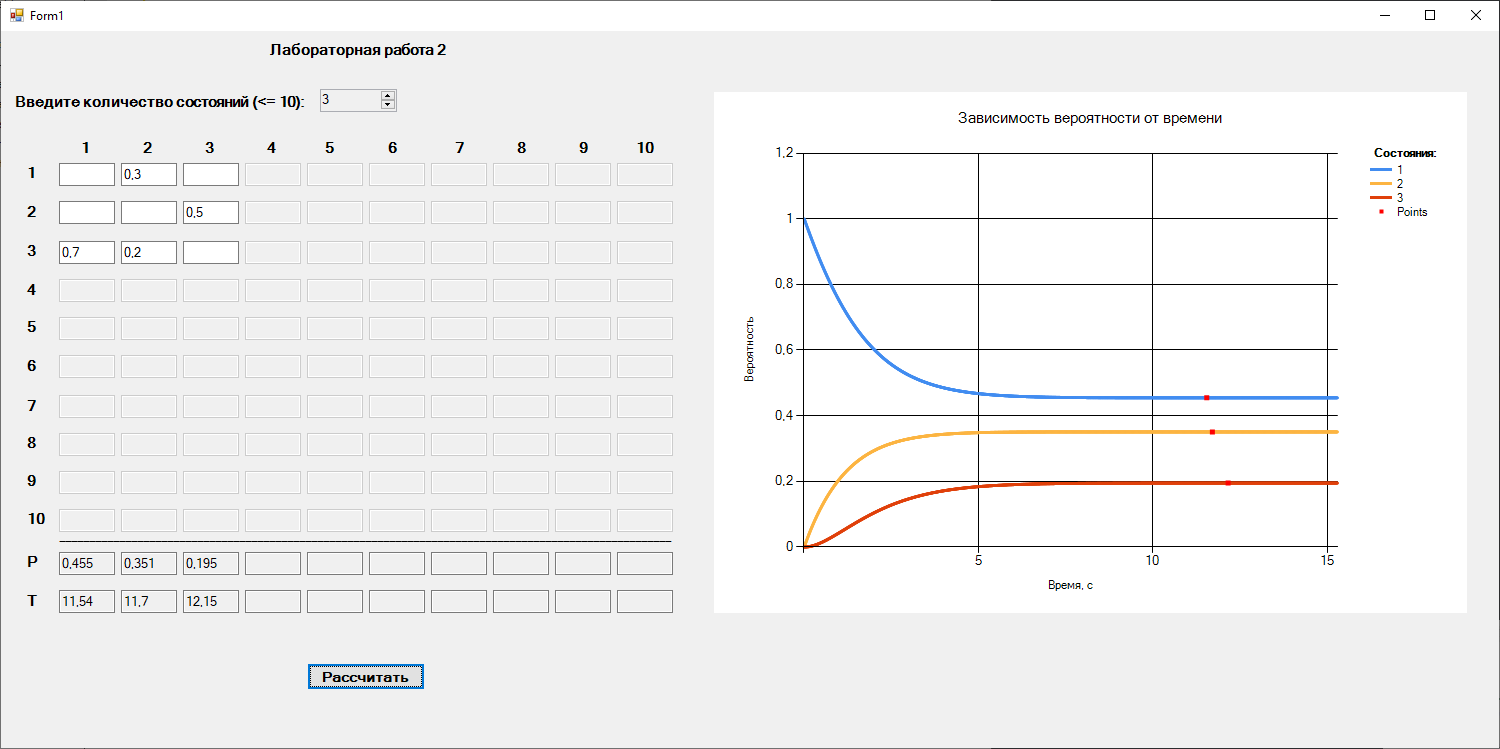
\includegraphics[scale = 0.42]{img/ex1_3.png}}
		\caption{Пример 1 (3 состояния)}
		\label{fig1:image}
	\end{center}
\end{figure}

Посчитаем $P_i$ самостоятельно:
\begin{equation}
	\left\{\begin{array}{l}
		0 = 0.7\cdot p_3 - 0.3\cdot p_1;\\
		0 = 0.3\cdot p_1 + 0.2\cdot p_3 - 0.5\cdot p_2;\\
		0 = 0.5\cdot p_2 - 0.2\cdot p_3 - 0.7\cdot p_3;\\
		p_1 + p_2 + p_3 = 1.
	\end{array}\right.
\end{equation}

\begin{equation}
	\left\{\begin{array}{l}
		p_1 = \frac{7}{3} p_3;\\
		p_2 = \frac{9}{5} p_3;\\
		\frac{7}{3} p_3 + \frac{9}{5} p_3 + p_3 = 1.
	\end{array}\right.
\end{equation}

\begin{equation}
	\left\{\begin{array}{l}
		p_1 \approx 0,4545 \approx 0,455;\\
		p_2 \approx 0,3506 \approx 0,351;\\
		p_3 \approx 0,1948 \approx 0,195.
	\end{array}\right.
\end{equation}

Результаты приблизительно равны. 

На Рис. \ref{fig2:image} представлен пример из лекции для 8 состояний. 

\begin{figure}[h]
	\begin{center}
		{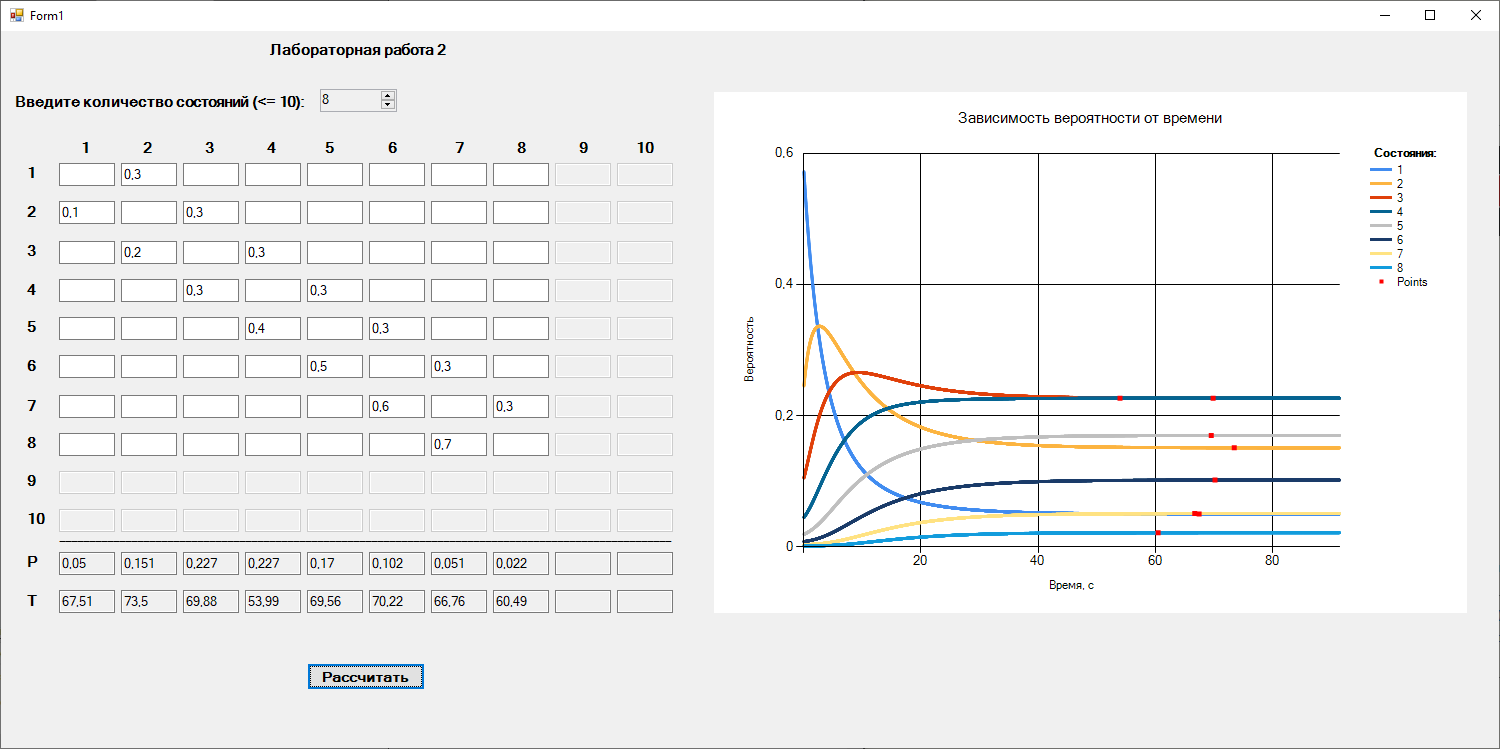
\includegraphics[scale = 0.42]{img/ex2_8.png}}
		\caption{Пример 2 (8 состояний)}
		\label{fig2:image}
	\end{center}
\end{figure}

\newpage

На Рис. \ref{fig3:image} представлен пример для 4 состояний, из последнего узла нет переходов в другие состояния. 

\begin{figure}[h]
	\begin{center}
		{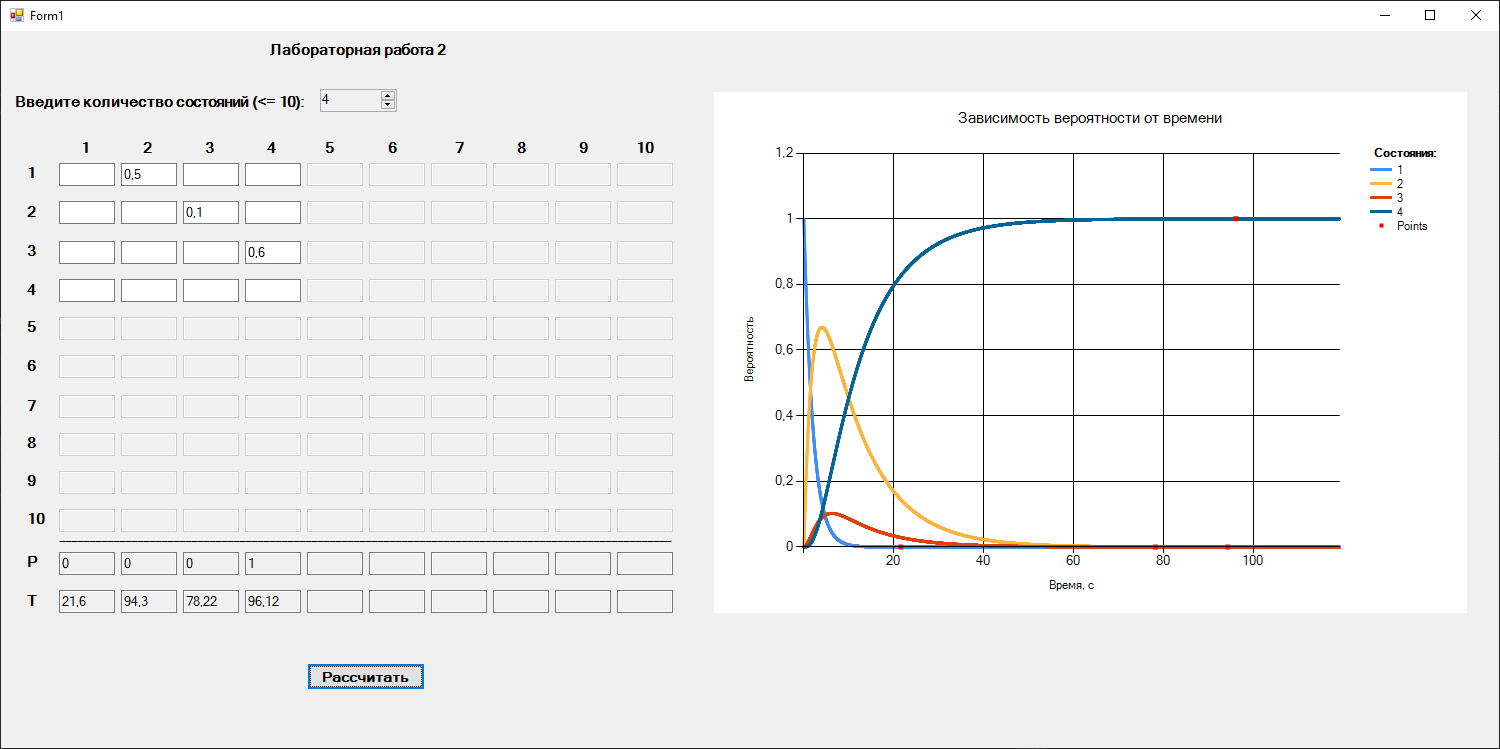
\includegraphics[scale = 0.42]{img/ex3_4.png}}
		\caption{Пример 3 (4 состояний)}
		\label{fig3:image}
	\end{center}
\end{figure}
\newpage

